\documentclass[12pt]{extarticle}
%Some packages I commonly use.
\usepackage[portuguese]{babel}
\usepackage{graphicx}
\usepackage{framed}
\usepackage[normalem]{ulem}
\usepackage{amsmath}
\usepackage{amsthm}
\usepackage{amssymb}
\usepackage{amsfonts}
\usepackage{enumerate}
\usepackage[utf8]{inputenc}
\usepackage{float}
\usepackage{gensymb}
\usepackage[top=1 in,bottom=1in, left=1 in, right=1 in]{geometry}
\usepackage{multirow}
\usepackage{float}
\usepackage{caption}
\usepackage{subcaption}
\usepackage{physics}
\usepackage[utf8]{inputenc}

%A bunch of definitions that make my life easier
\newcommand{\matlab}{{\sc Matlab} }
\newcommand{\cvec}[1]{{\mathbf #1}}
\newcommand{\rvec}[1]{\vec{\mathbf #1}}
\newcommand{\ihat}{\hat{\textbf{\i}}}
\newcommand{\jhat}{\hat{\textbf{\j}}}
\newcommand{\khat}{\hat{\textbf{k}}}
\newcommand{\minor}{{\rm minor}}
\newcommand{\trace}{{\rm trace}}
\newcommand{\spn}{{\rm Span}}
\newcommand{\rem}{{\rm rem}}
\newcommand{\ran}{{\rm range}}
\newcommand{\range}{{\rm range}}
\newcommand{\mdiv}{{\rm div}}
\newcommand{\proj}{{\rm proj}}
\newcommand{\R}{\mathbb{R}}
\newcommand{\N}{\mathbb{N}}
\newcommand{\Q}{\mathbb{Q}}
\newcommand{\Z}{\mathbb{Z}}
\newcommand{\<}{\langle}
\renewcommand{\>}{\rangle}
\renewcommand{\emptyset}{\varnothing}
\newcommand{\attn}[1]{\textbf{#1}}
\theoremstyle{definition}
\newtheorem{theorem}{Theorem}
\newtheorem{corollary}{Corollary}
\newtheorem*{definition}{Definition}
\newtheorem*{example}{Example}
\newtheorem*{note}{Note}
\newtheorem{exercise}{Exercise}
\newcommand{\bproof}{\bigskip {\bf Proof. }}
\newcommand{\eproof}{\hfill\qedsymbol}
\newcommand{\Disp}{\displaystyle}
\newcommand{\qe}{\hfill\(\bigtriangledown\)}
\setlength{\columnseprule}{1 pt}
\usepackage[utf8]{inputenc}

\title{Análise Gráfica e Movimento Circular}
\author{Felipe Salvador}
\date{Atualizado em \today}

\begin{document}

\maketitle

Na aula de hoje, iremos entender como funciona a análise de gráficos e como extrair as informações de um gráfico dado. Na segunda parte, iremos tratar sobre uma entidade matemática chamada vetores, que iremos usar nas próximas aulas.

\section{Análise Gráfica}

Uma das formas que um exercício dá informações é por meio de gráficos, pois além de ser bem sucinto, é uma forma bem visual de expor informações que, em forma de texto, ficaria difícil de compreender. Para isso, vamos agora aprender como se lê gráficos e como as informações são embutidas neles.

A primeira parte que temos que olhar no gráfico é que tipo de informações estão sendo dadas ali. Para isso, olhamos para \textbf{os eixos do gráficos.} Eles são 2:

\begin{itemize}
    \item \textbf{O eixo das abscissas (ou eixo X)} - ele dá as informações na horizontal;
    \item \textbf{O eixo das ordenadas (ou eixo Y)} - ele dá as informações na vertical.
\end{itemize}

Assim como no jogo Batalha Naval, o cruzamento de 1 informação do eixo das abscissas com 1 informação do eixo das ordenadas resulta em \textbf{1 ponto} no gráfico. \textbf{Então, sempre que vermos 1 ponto no gráfico, ele indica DUAS informações, uma em cada eixo.} Veja a figura \ref{fig:graph_basics} para ver visualmente o que foi dito acima.

\begin{figure}[H]
    \centering
    \begin{subfigure}[b]{0.4\textwidth}
         \centering
         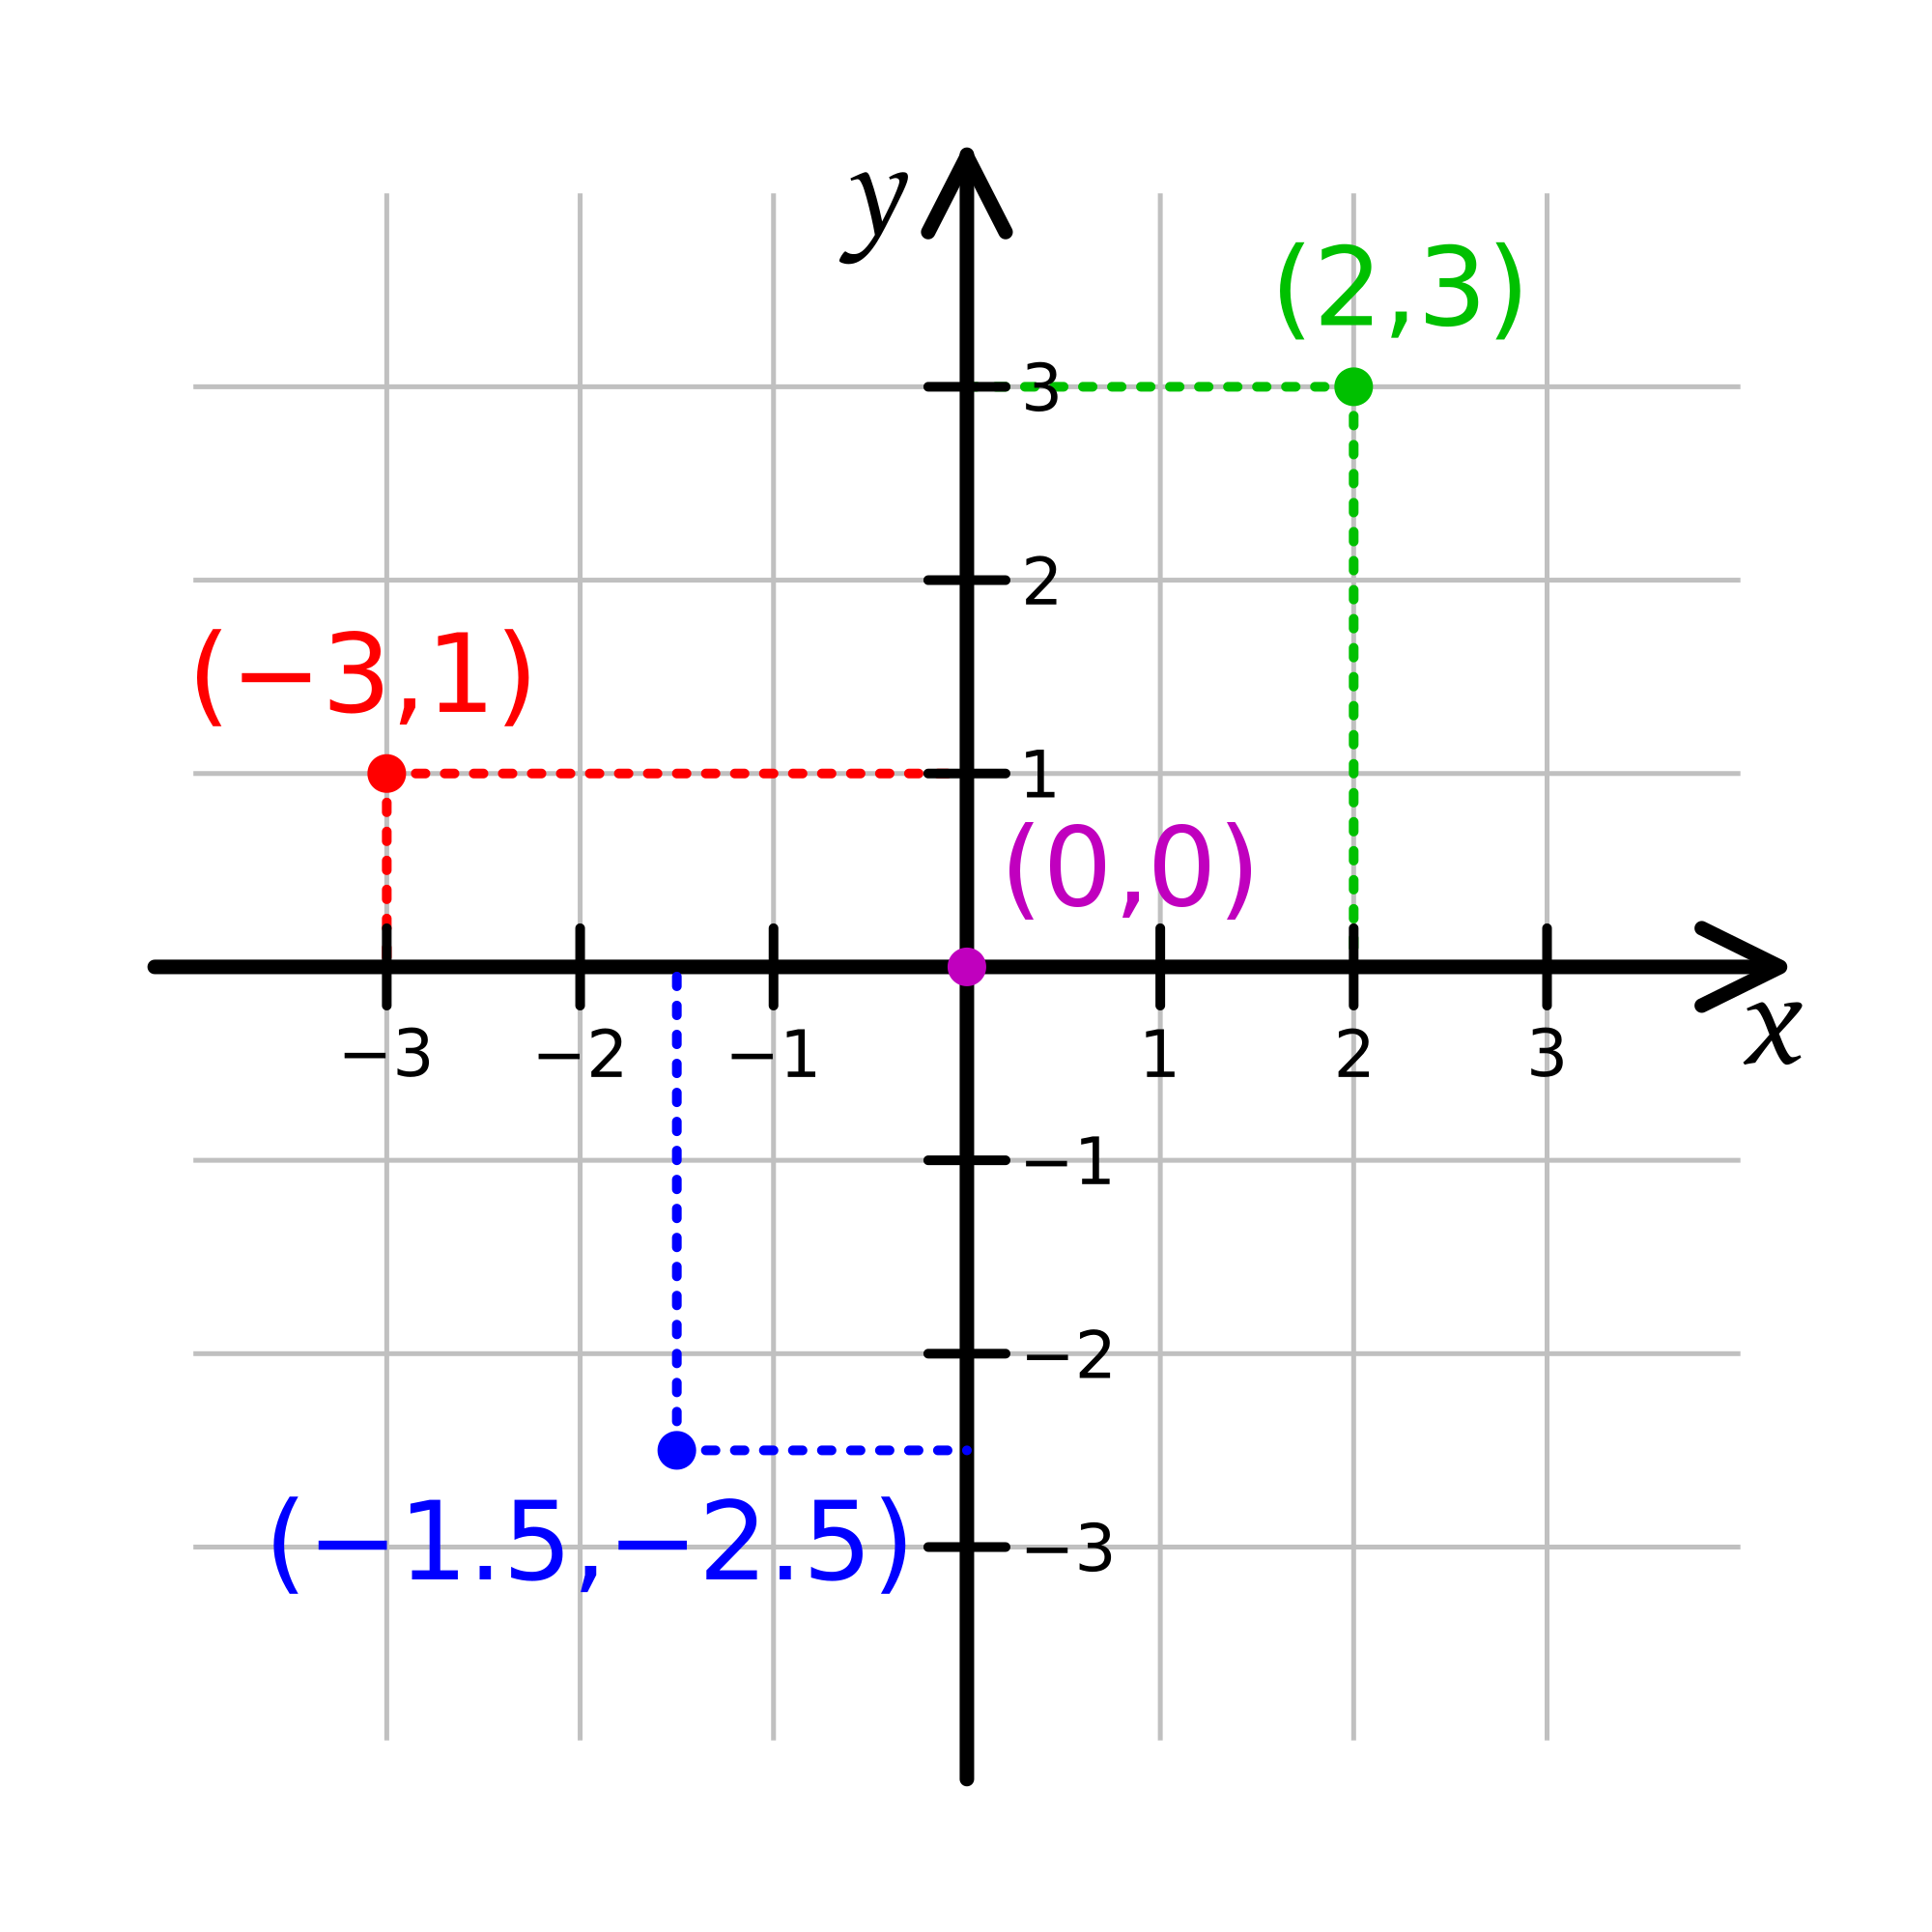
\includegraphics[width=\textwidth]{2000px-Cartesian-coordinate-system.svg.png}
         \caption{Esse gráfico está mostrando um conjunto de pontos, em que cada ponto dá a informação da sua posição no eixo Y e no eixo X}
         \label{fig:graph_point}
     \end{subfigure}
     \hfill
     \begin{subfigure}[b]{0.4\textwidth}
         \centering
         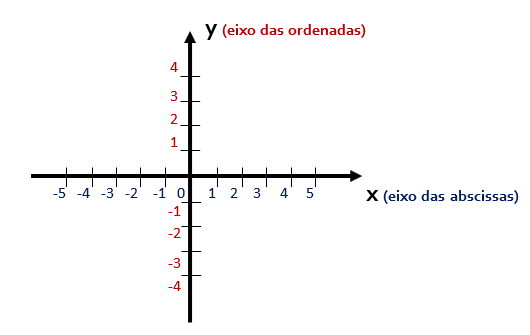
\includegraphics[width=1\textwidth]{T3-eixo-das-abscissas-e-das-ordenadas-no-plano-cartesiano.png}
         \caption{Esquema sobre os eixos de um gráfico}
         \label{fig:eixos}
     \end{subfigure}
     \caption{2 figuras que demonstram as características de um gráfico - os seus eixos e como as informações são postas.}
     \label{fig:graph_basics}
\end{figure}

A partir disso, vamos povoando o gráfico com as informações que temos, lembrando que precisamos sempre de um par de informações (1 de cada eixo) para que possamos colocar no gráfico. As vezes, vemos que no gráfico, não há pontos, mas sim uma reta ou uma curva nele. \textbf{Isso significa que os pontos estão tão próximos um do outro que eles formam essa linha ou curva.}

Isso nos diz bastante sobre o comportamento da informação dada. Como no exemplo da figura \ref{fig:graph_plots}, que mostram a posição de 2 objetos em relação ao tempo. Perceba que não vemos pontos, mas uma linha indicando que os pontos estão tão próximos um do outro, formando uma linha contínua.
\begin{figure}[H]
    \centering
    \begin{subfigure}[b]{0.4\textwidth}
         \centering
         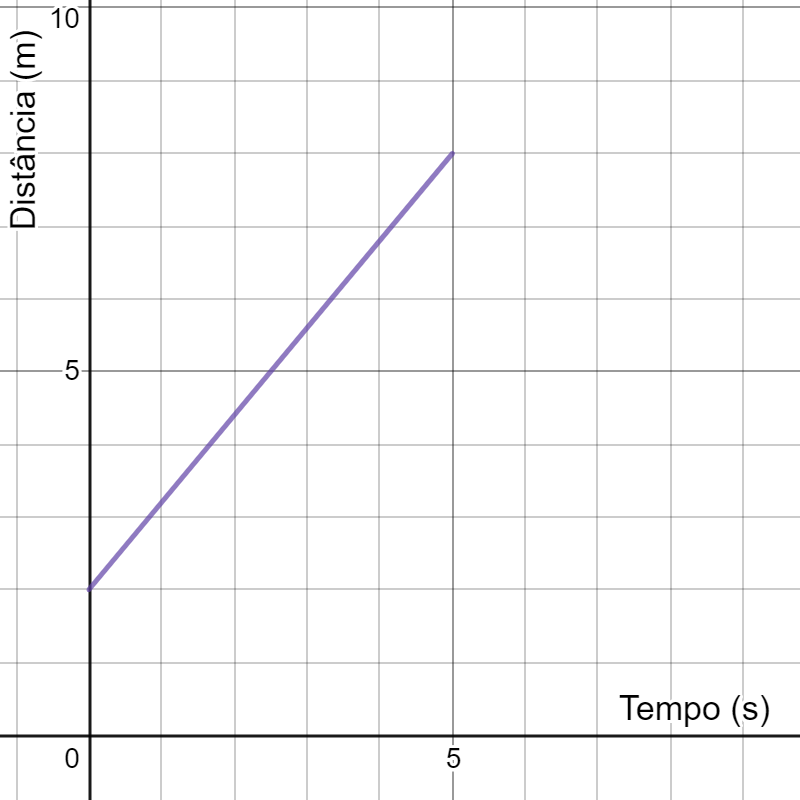
\includegraphics[width=\textwidth]{line.png}
         \caption{Esse gráfico está mostrando a posição de uma pessoa ao longo do tempo}
         \label{fig:line}
     \end{subfigure}
     \hfill
     \begin{subfigure}[b]{0.4\textwidth}
         \centering
         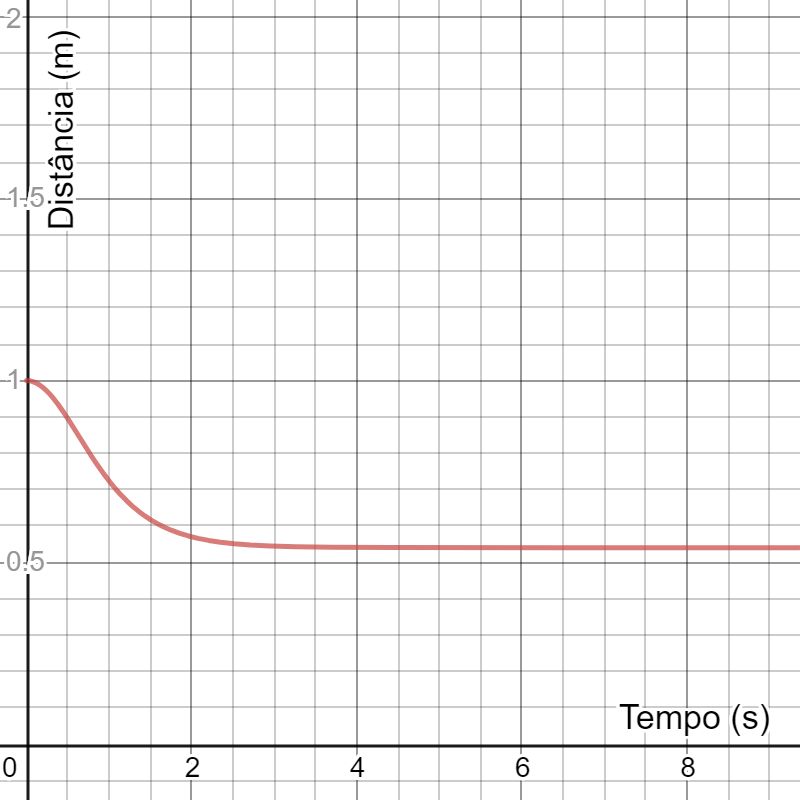
\includegraphics[width=\textwidth]{curve.png}
         \caption{Esse gráfico está mostrando a posição de um carro ao longo do tempo}
         \label{fig:curve}
     \end{subfigure}
     \caption{Exemplo de gráficos que mostram retas ou curvas, indicando que os pontos estão perto um do outro que eles formam uma linha contínua.}
     \label{fig:graph_plots}
\end{figure}

Muito bem, agora vamos aprender a extrair informações de gráficos que são segmentos de reta. Nessa parte, iremos usar alguns conceitos de Geometria Analítica, então caso você ainda não tenha se familiarizado com as fórmulas dadas, não se preocupe que você verá mais para frente de onde vem.

O primeiro conceito é que a reta de um gráfico é descrita por:
\begin{equation}\label{eq:reta}
    y = m.x + b
\end{equation}
em que, '$y$' é a informação dada no eixo Y, '$x$' é a informação dada no eixo X, '$m$' é chamado de \textbf{coeficiente angular} e '$b$' de \textbf{coeficiente linear}.

O primeiro ponto a ser ressaltado na equação (\ref{eq:reta}) é que \textbf{se $x=0$, então $y=b$}. \textbf{Ou seja, o valor da coordenada no eixo Y quando a reta cruza o eixo Y, é o valor do coeficiente linear $b$.}

Essa informação sobre a reta é bem direta e independe de quaisquer outras informações que estejam dados no gráfico. Isso ajuda-nos a construir a equação que descreve a reta sem muitos problemas.

Já o coeficiente angular é dado a partir da seguinte equação:

\begin{equation}\label{eq:angular}
    m = \frac{y_B - y_A}{x_B - x_A}
\end{equation}
em que $y_B$ e $y_A$ são informações do eixo Y sobre 2 pontos dados da reta, enquanto $x_B$ e $x_A$ são as informações do eixo X sobre esses 2 pontos. A figura (\ref{fig:coef_ang}) demonstra visualmente o que essa equação nos diz:
\begin{figure}[H]
    \centering
    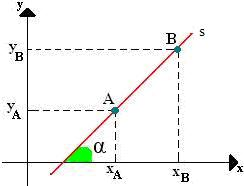
\includegraphics[width=0.5\textwidth]{cauculo coefi1.jpg}
    \caption{Esquema visual de o que é o coeficiente angular $m$ da equação de uma reta. A e B são pontos da reta em que as suas coordenadas do eixo X e Y são dadas como $x_A$ e $y_A$ para o ponto A e $x_B$ e $y_B$ para o ponto B.}
    \label{fig:coef_ang}
\end{figure}

Um ponto importante que é consequência da equação (\ref{eq:angular}) é que $m$ tem a seguinte unidade:
\begin{equation}
    [m] = \frac{\text{[unidade do eixo Y]}}{\text{[unidade do eixo X]}}
\end{equation}

Então, na figura \ref{fig:line}, o eixo Y designa distância em metros (m) e o eixo X designa tempo em segundos (s), portanto:
\begin{equation}
    [m] = \frac{m}{s}
\end{equation}

\textbf{Logo, o coeficiente angular da figura \ref{fig:line} tem a informação da velocidade média ($v$) que o meu objeto fez durante o percurso dele.}

Na mesma figura \ref{fig:line}, a reta cruza com o eixo Y em $y=2$, logo em $t=0$ (onde tudo começou), o meu objeto estava na posição de 2 metros longe da origem.

As vezes, temos que tirar um outro tipo de informação mais sutil. A operação que iremos fazer então será \textbf{calcular a área debaixo da reta dada.\footnote{Para aqueles que forem seguir o caminho das exatas, na faculdade, vocês irão ver em Cálculo 1, que esse procedimento se chama \textit{Integração de uma função}. Mas por enquanto, é somente calcular a área debaixo de um gráfico =) }} Vamos usar como exemplo a figura (\ref{fig:vel_ex}):
\begin{figure}[H]
    \centering
    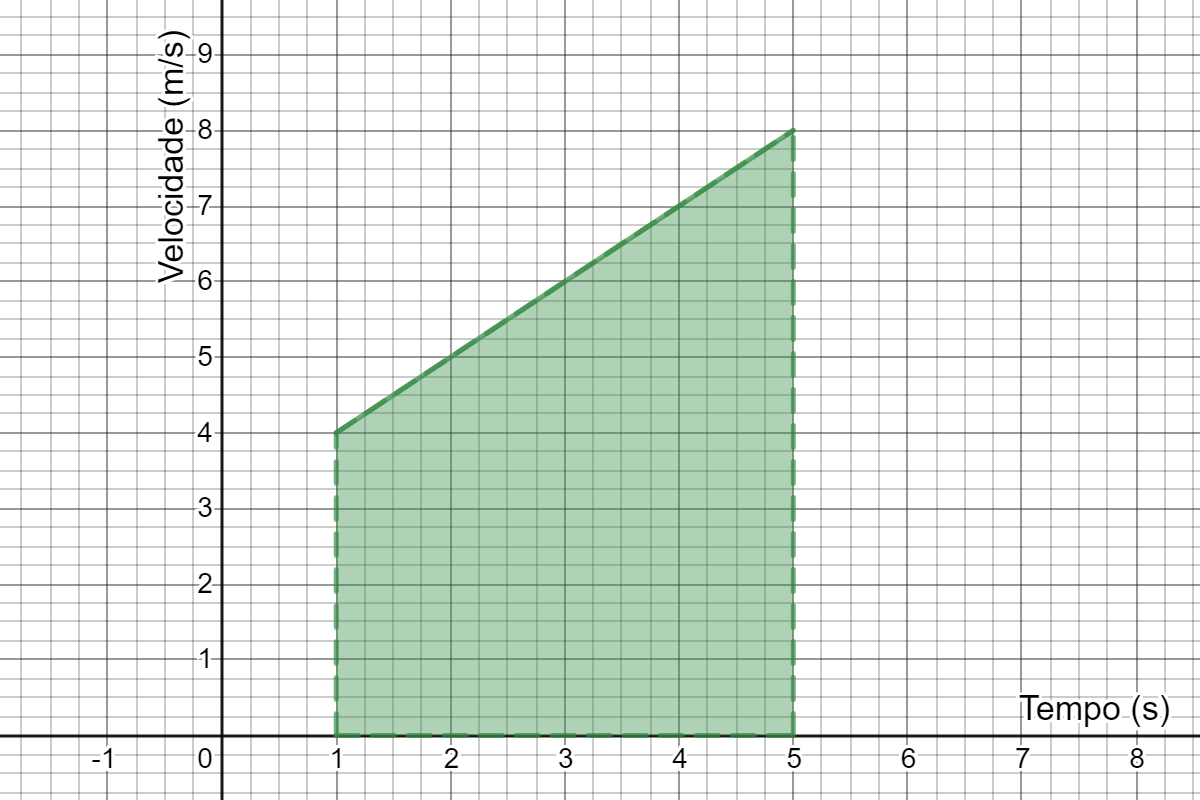
\includegraphics[width=0.5\textwidth]{area_under.png}
    \caption{Gráfico da velocidade em relação ao tempo}
    \label{fig:vel_ex}
\end{figure}

Perceba que a figura pintada é um trapézio (\textit{caso não esteja vendo vire a cabeça de lado e olhe o gráfico}), então a área debaixo de um gráfico é dada pela fórmula da área de um trapézio:
\begin{equation}
    A = \frac{(b+B)*h}{2}
\end{equation}
em que '$b$' e '$B$' são os tamanhos das bases menor e maior, respectivamente. '$h$' é a altura do trapézio. \textbf{ATENÇÃO: os comprimentos das bases está dado nas informações do eixo Y !!!! No eixo X, o que é dado é a informação sobre a altura do trapézio '$h$'.}

Vamos calcular a área debaixo desse gráfico, então. Veja que a base menor desse gráfico tem tamanho 4, a base maior tem tamanho 8, e a altura desse trapézio é 5-1 = 4. Colocando essas informações na fórmula, temos que:

\begin{equation}
    A = \frac{(4+8)4}{2} = \frac{12*4}{2} = 24
\end{equation}

Agora, olhemos a unidade dessa conta. Os tamanhos das bases é dado em $m/s$, enquanto a altura é em $s$. Como na fórmula a soma das bases multiplica a altura, então temos que:
\begin{equation}\label{eq:area}
    [A] = [\text{unidade do eixo Y}]*[\text{unidade do eixo X}] = \frac{m}{s}*s = m
\end{equation}

Portanto, essa área tem unidade de comprimento (m), logo \textbf{essa área debaixo do gráfico nos dá a informação da distância percorrida.}

\textbf{Um ponto importante é que a unidade da área debaixo do gráfico é sempre o produto das unidades dos eixos X com a do eixo Y.}

Obs: \textit{nem sempre a figura feita pela área debaixo do gráfico é um trapézio. Pode ser um retângulo, quadrado ou até um triângulo. Então é importante fazer essas linhas tracejadas dos pontos dados até o eixo X para ver qual é a figura formada pela área.}

\subsection{Tipos de gráficos para cada tipo de movimento e conta a ser feita}
\begin{itemize}
    \item \textbf{Movimento Retilíneo Uniforme (MRU)}
    
    No MRU, temos a seguinte equação:
    \begin{equation}
        S = S_0 + v.t
    \end{equation}
    \begin{figure}[H]
    \centering
    \begin{subfigure}[b]{0.4\textwidth}
         \centering
         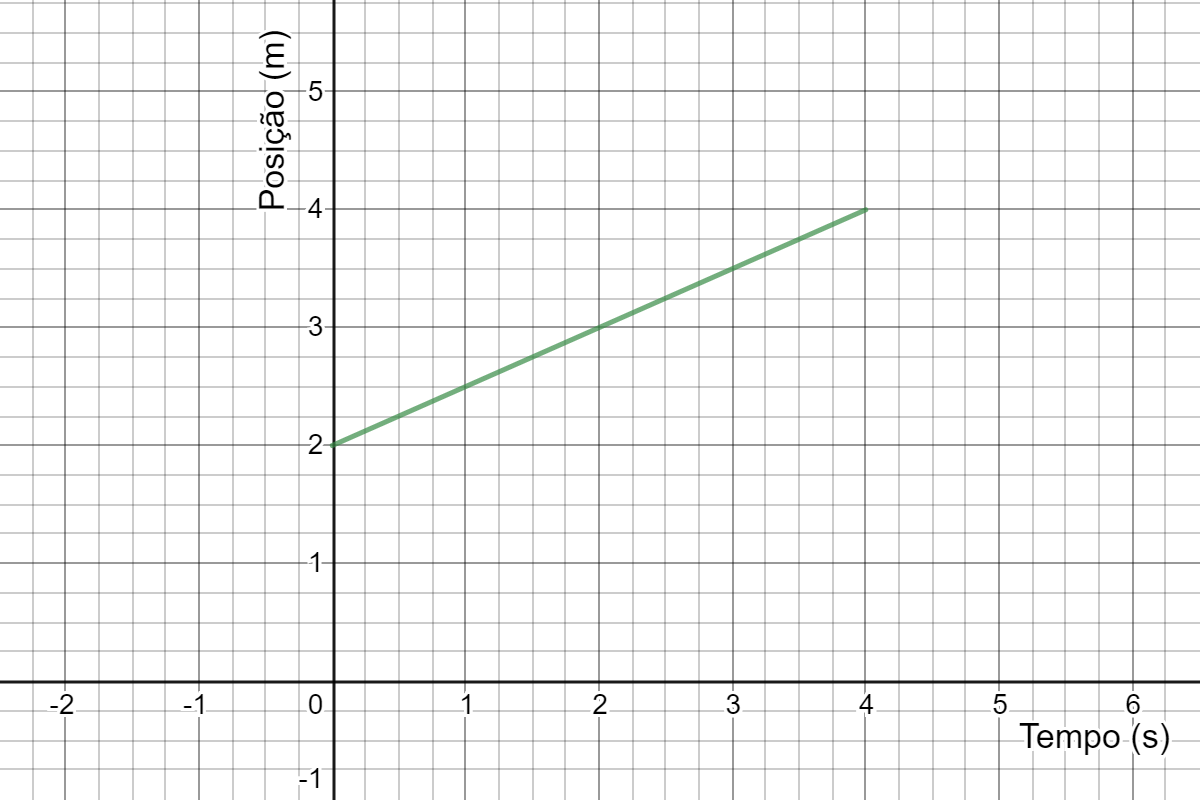
\includegraphics[width=\textwidth]{pos_MRU.png}
         \caption{Gráfico da posição em termos do tempo. Objetivo - calcular o coeficiente angular para achar a velocidade}
         \label{fig:MRU_vel}
     \end{subfigure}
     \hfill
     \begin{subfigure}[b]{0.4\textwidth}
         \centering
         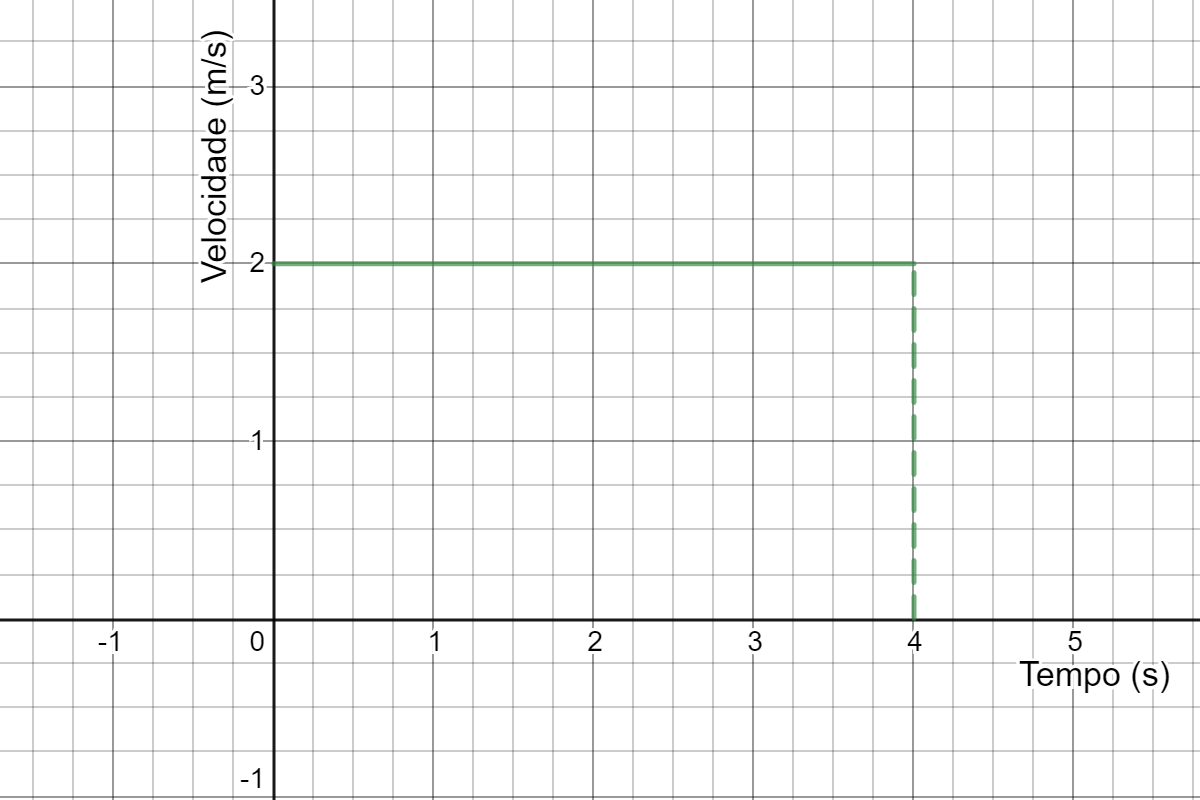
\includegraphics[width=\textwidth]{MRU_v.png}
         \caption{Gráfico da velocidade em termos do tempo de um Movimento Retilíneo Uniforme (MRU). Objetivo - calcular a área debaixo do gráfico (área do retângulo ou quadrado) para achar a distância percorrida no intervalo de tempo dado.}
         \label{fig:MRU_pos}
     \end{subfigure}
     \caption{Gráficos do Movimento Retilíneo Uniforme (MRU). O gráfico de velocidade por tempo é sempre uma \textbf{reta horizontal} e o gráfico de posição por tempo é sempre uma \textbf{reta diagonal} (para cima ou para baixo).}
     \label{fig:MRU_plots}
\end{figure}

\item \textbf{Movimento Uniformemente Variado (MUV)}

Lembrando que no MUV, as equações sobre o espaço e velocidade são dadas por:

\begin{align}
    &S = S_0 +v_0.t + \frac{a.t^2}{2}\quad\text{(Equação horária do Espaço (Sorvetão))}\\
    &v= v_0 + a.t \quad\text{(Equação da velocidade)}\\ 
    &v^2 = v_0^2 + 2.a.\delta S \quad\text{(Equação de Torricelli)}
\end{align}
        \begin{figure}[H]
    \centering
    \begin{subfigure}[b]{0.4\textwidth}
         \centering
         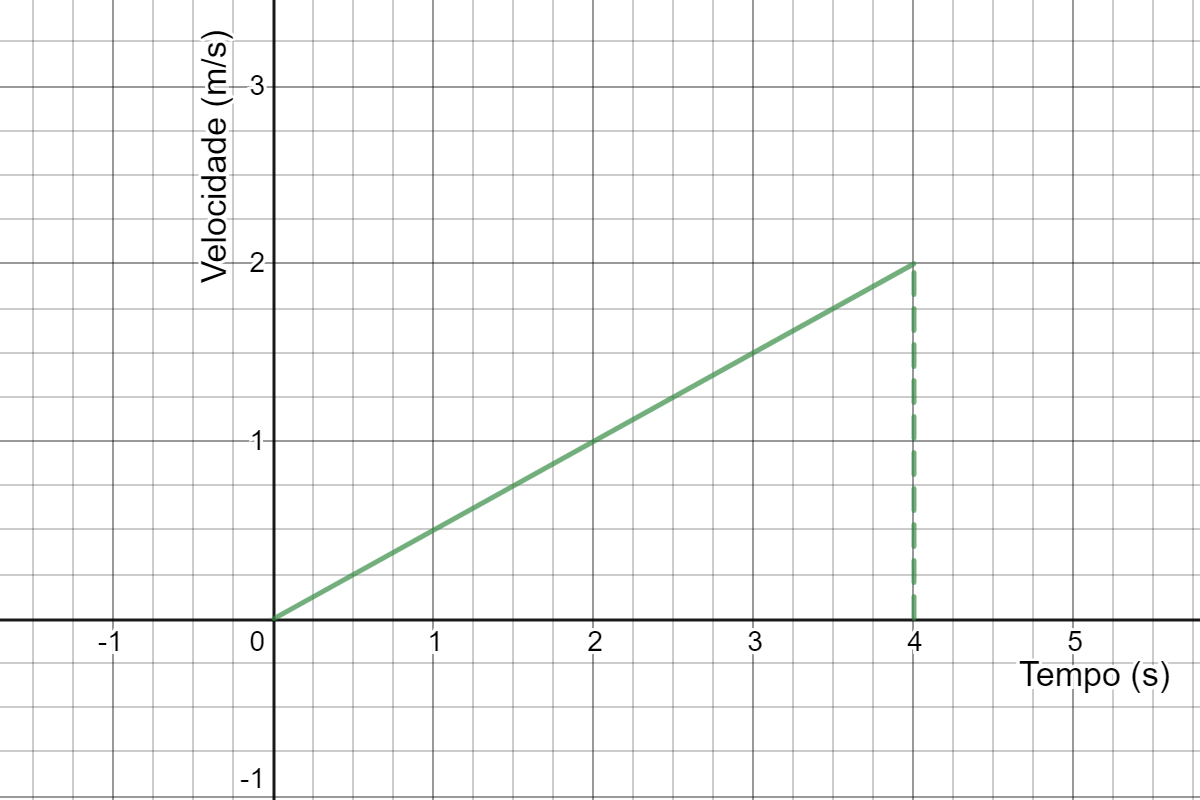
\includegraphics[width=\textwidth]{MUV_vel.png}
         \caption{Gráfico da velocidade em termos do tempo de um Movimento Uniformemente Variado (MUV). Objetivo - calcular o coeficiente angular para achar a aceleração OU calcular a área debaixo do gráfico para achar a distância percorrida}
         \label{fig:MUV_vel}
     \end{subfigure}
     \hfill
     \begin{subfigure}[b]{0.4\textwidth}
         \centering
         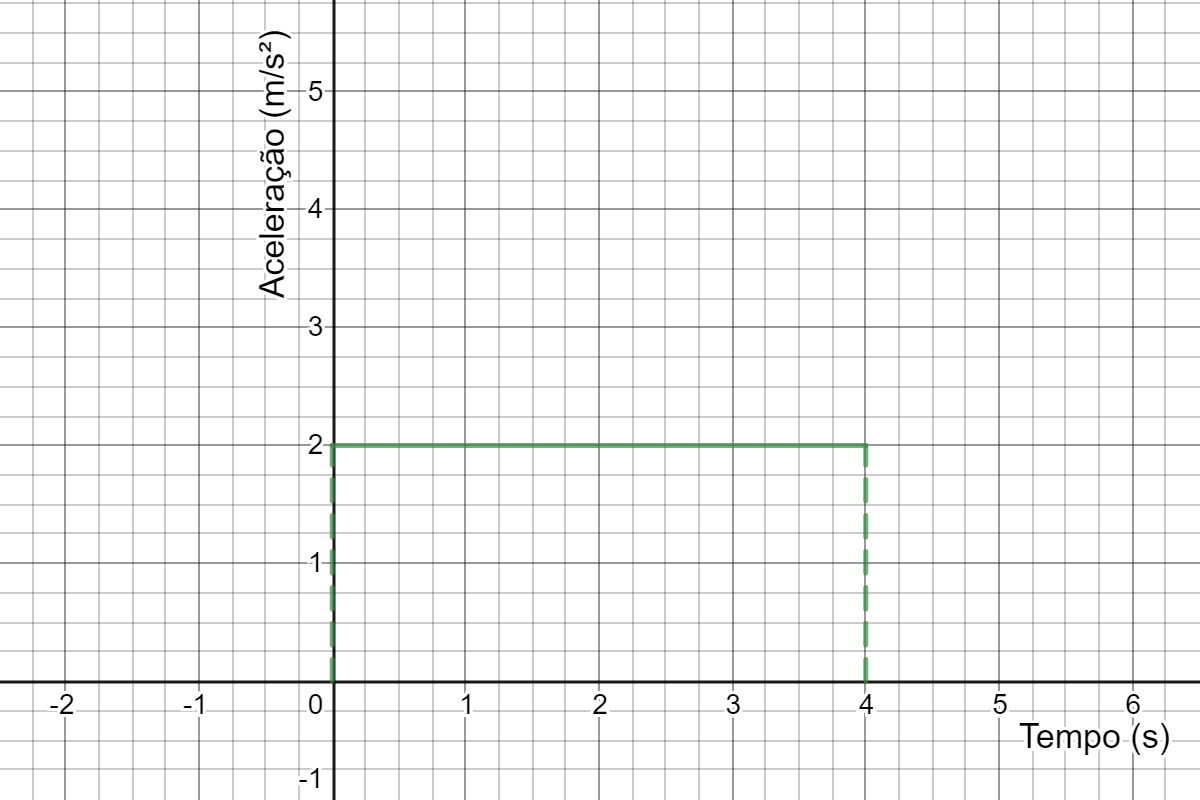
\includegraphics[width=\textwidth]{aceleracao_MUV.png}
         \caption{Gráfico da aceleração em termos do tempo de um Movimento Uniformemente Variado (MUV). Objetivo - calcular a área debaixo do gráfico (área do retângulo ou quadrado) para achar a variação da velocidade ($\Delta v$), ou seja, a velocidade final - velocidade inicial.}
         \label{fig:MRU_pos}
     \end{subfigure}
     \\
     \begin{subfigure}[b]{0.4\textwidth}
         \centering
         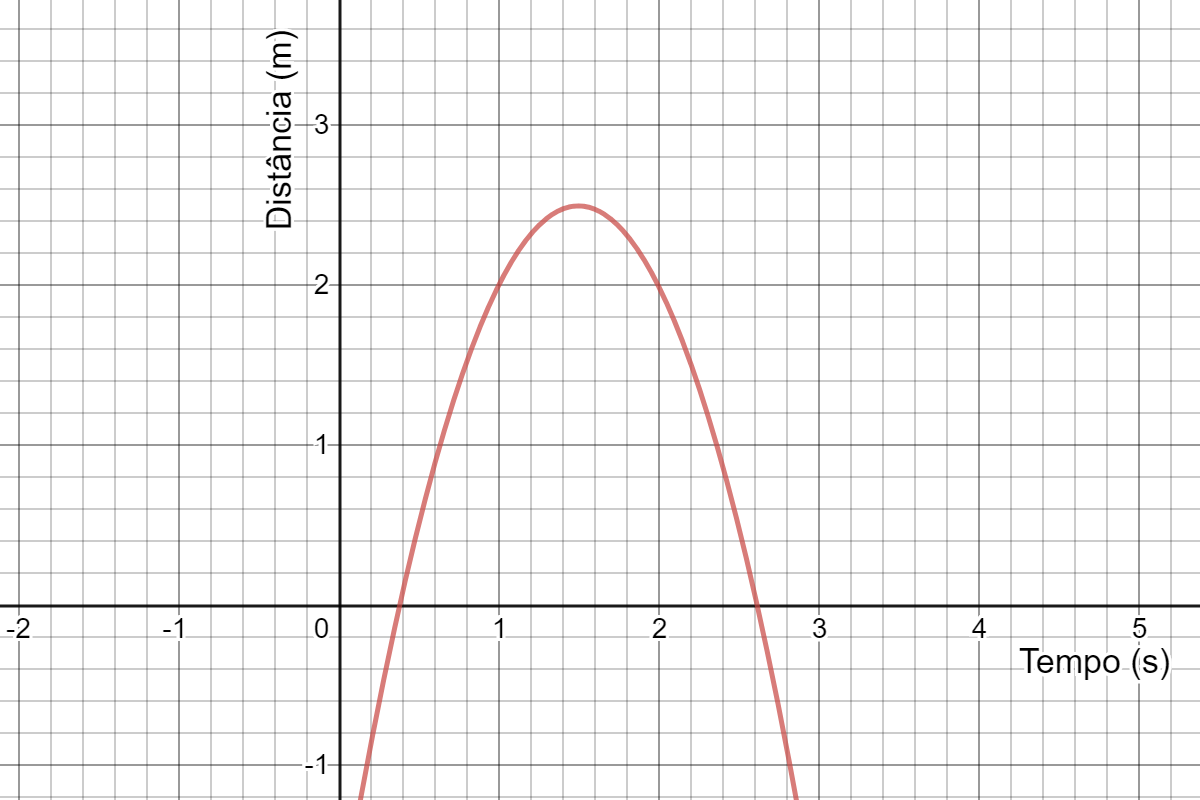
\includegraphics[width=\textwidth]{pos_a_neg.png}
         \caption{Gráfico da posição em termos do tempo de um Movimento Uniformemente Variado (MUV). Perceba que o gráfico é uma parábola com concavidade virada para baixo. \textbf{Então, a aceleração que o objeto sobre é negativa!!!}}
         \label{fig:MUV_pos_a<0}
     \end{subfigure}
     \hfill
     \begin{subfigure}[b]{0.4\textwidth}
         \centering
         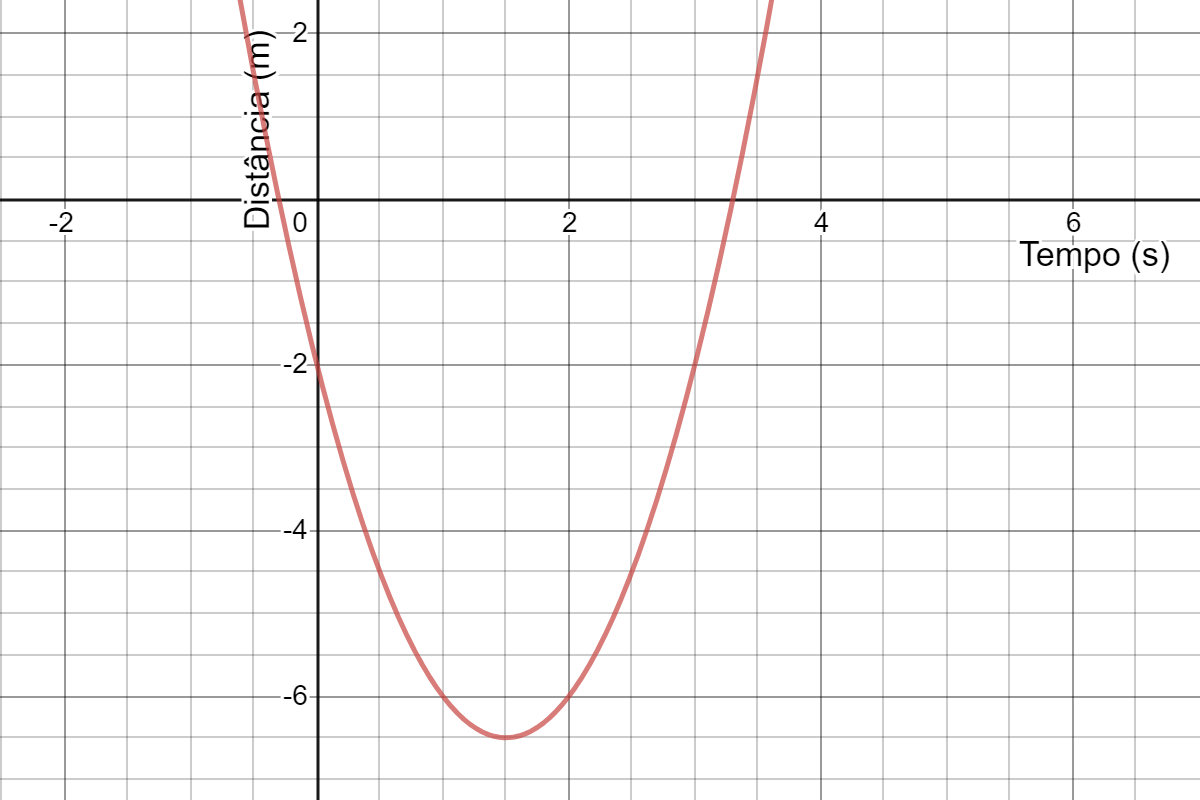
\includegraphics[width=\textwidth]{pos_a_pos.png}
         \caption{Gráfico da posição em termos do tempo de um Movimento Uniformemente Variado (MUV). Perceba que o gráfico é uma parábola com concavidade virada para cima. \textbf{Então, a aceleração que o objeto sobre é positiva!!!}}
         \label{fig:MUV_pos_a>0}
     \end{subfigure}
     \caption{Gráficos do Movimento Retilíneo Uniforme (MRU). O gráfico de velocidade por tempo é sempre uma \textbf{reta horizontal} e o gráfico de posição por tempo é sempre uma \textbf{reta diagonal} (para cima ou para baixo).}
     \label{fig:MRU_plots}
\end{figure}
\end{itemize}

\section{Vetores}

Antes de entrar nas últimas partes sobre a cinemática, vamos dar uma pausa para explicar vetores que será necessário para terminar o assunto de cinemática e muito útil para a próxima matéria que será dinâmica.

Mas antes, vamos diferenciar o que é um vetor de um escalar:
\begin{itemize}
    \item \textbf{Escalar} - são números que podem ou não ter unidades envolvidas. Podem ser positivos ou negativos. \textit{Ex: Temperatura, tempo}
    \item \textbf{Vetor} - são quantidades que tem \textbf{direção, sentido e módulo}. Com direção, eu quero dizer que tem um lugar para onde aponta. Com sentido, eu quero dizer que para qual lado está apontado, ex: para cima ou para baixo. Com módulo, eu quero dizer o tamanho ou a intensidade que isso tem. \textit{Ex: posição, velocidade}
\end{itemize}

A forma mais conhecida de se ilustrar um vetor é por meio de uma flecha:
\begin{figure}[H]
    \centering
    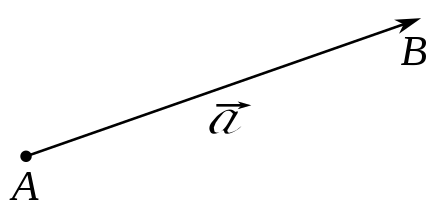
\includegraphics[width=0.3\textwidth]{440px-VectorAB.svg.png}
    \caption{Ilustração de o que é um vetor. A linha da flecha representa a direção, a ponta da flecha representa o sentido e o tamanho da flecha representa o módulo.}
    \label{fig:vector}
\end{figure}

Na representação de um vetor por meio da flecha, \textbf{a linha é a direção, a ponta da flecha é o sentido e o tamanho da flecha é o módulo.} Sempre que falamos de vetores, essas 3 características estão envolvidas.

A necessidade de se ter um formalismo vetorial vem do fato que certas quantidades, como a velocidade, dependem de mais informações do que quão grande elas são. Por que quando fala que está a 50 km/h, uma possível pergunta é "para qual direção?", pois está indo a 50km/h em direção a você significa que a pessoa está se aproximando, enquanto se estiver indo no sentido oposto ao seu, ela está se afastando. Qualquer coisa diferente, significa que ela está indo a um outro lugar.

Mas, temos uma aula só de vetores por causa de uma questão. \textbf{Vetores são operados de forma levemente diferente do que números.} Temos algumas regras importantes que temos que respeitar para que o seu resultado seja o resultado real.

\subsection{Notação vetorial}

O primeiro fato vem de como diferenciamos um vetor de um escalar (número). A primeira questão é que vetor SEMPRE se escreve com uma flecha sobre a letra ou expressão que o designa:
\begin{equation}
    \va{a}
\end{equation}

Existe uma outra notação para quando está escrito via texto online que é colocar o símbolo em negrito como: $\mathbf{a}$. Não é comum para Ensino Médio essa notação, mas pode ser que vocês esbarrem nessa notação em livros e pela Internet.

Lembrando que a flecha sobre o simbolo faz parte do personagem vetor, ou seja, sempre que tiver flecha em cima do símbolo é um vetor e o contrário também.

\section{Operação com vetores (soma, subtração, comprimento e multiplicação por escalar)}

Aqui está o conteúdo mais importante sobre vetores. Saber operar eles é crucial para qualquer teoria que usa eles e vamos aqui nessa parte descrever parcial o que se dá para fazer com vetores. \footnote{Para aqueles que vão entrar na jornada das exatas, vocês verão que existe outras operações como produto escalar ($<\vdot>$) e produto vetorial ($<\cross>$). Lembra que a \textit{tia} do ensino fundamental usava $\cross$ como símbolo de multiplicação e de uma hora para outra começou a usar o $\vdot$ ? É por isso =)} Nessa parte, só iremos aprender a usar o que vamos precisar.

Primeiramente, um vetor é descrito de forma matemática como:

\begin{equation}
    \va{a} = (a_1, a_2)
\end{equation}
em que $a_1,\,a_2$ são números. \textbf{Esses 2 números descrevem onde a ponta da flecha aponta e o início da flecha sempre estará na origem, que é o (0,0).} Para ter uma visão sobre como essa forma de escrever o vetor se relaciona com a flecha, veja abaixo:

\begin{figure}[H]
    \centering
    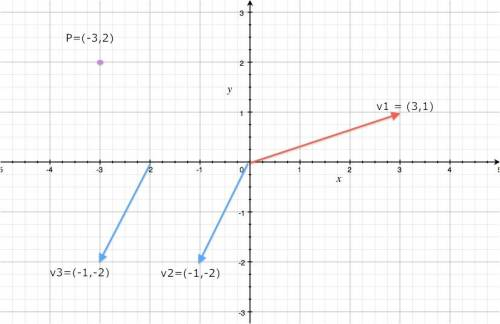
\includegraphics[width=0.7\textwidth]{vectors.jpg}
    \caption{Exemplos de vetores num plano sendo descritos por flechas. A representação de v3 não está correta!!!}
    \label{fig:vectors}
\end{figure}

\subsection{Soma de vetores (+)}

A primeira operação que fazemos com vetores é a de soma (+). Ela definida da seguinte forma:

Dados 2 vetores, definido como: $\va{a} = (a_1,a_2)$ e $\va{b} = (b_1,b_2)$, a soma de vetores $\va{a} + \va{b}$ é definida como:
\begin{equation}
    \boxed{\va{a} + \va{b} = (a_1+b_1, a_2+b_2)}
\end{equation}

\textbf{Perceba que os índices não se misturam}. As entradas dos vetores com primeiros índices são somados entre si e a mesma coisa para os segundos índices.

Em termos da flecha, a soma de vetores é dada pela \textbf{Regra do Paralelogramo}:

\begin{figure}[H]
    \centering
    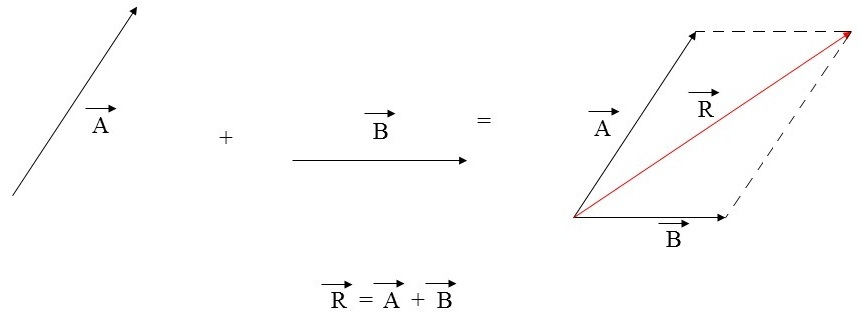
\includegraphics[width=0.8\textwidth]{5863e9ecd787d-vetores.jpg}
    \caption{Regra do Paralelogramo - você copia o vetor $\va{A}$ e coloca ele na ponta do vetor $\va{B}$, fazendo a mesma coisa com o $\va{B}$ colocando na ponta do vetor $\va{A}$. Após isso, você vê onde as duas pontas da flecha se cruzam e traça um vetor partindo de onde os dois começam e indo até onde as pontas se tocam.}
    \label{fig:sum_vectors}
\end{figure}

A regra diz que a soma de 2 vetores é descrita pelo vetor que parte de onde os 2 vetores partem e chega até as pontas deles se encontram. O nome da regra vem da forma geométrica que esse método faz - um paralelogramo.

\textit{Exemplo:} Seja $\va{a} = (1,1)$ e $\va{b} = (3,1)$:
\begin{equation}
    \va{a} + \va{b} = (1+3,1+1) = (4,2)
\end{equation}

Na representação das flechas, fica assim:
\begin{figure}[H]
    \centering
    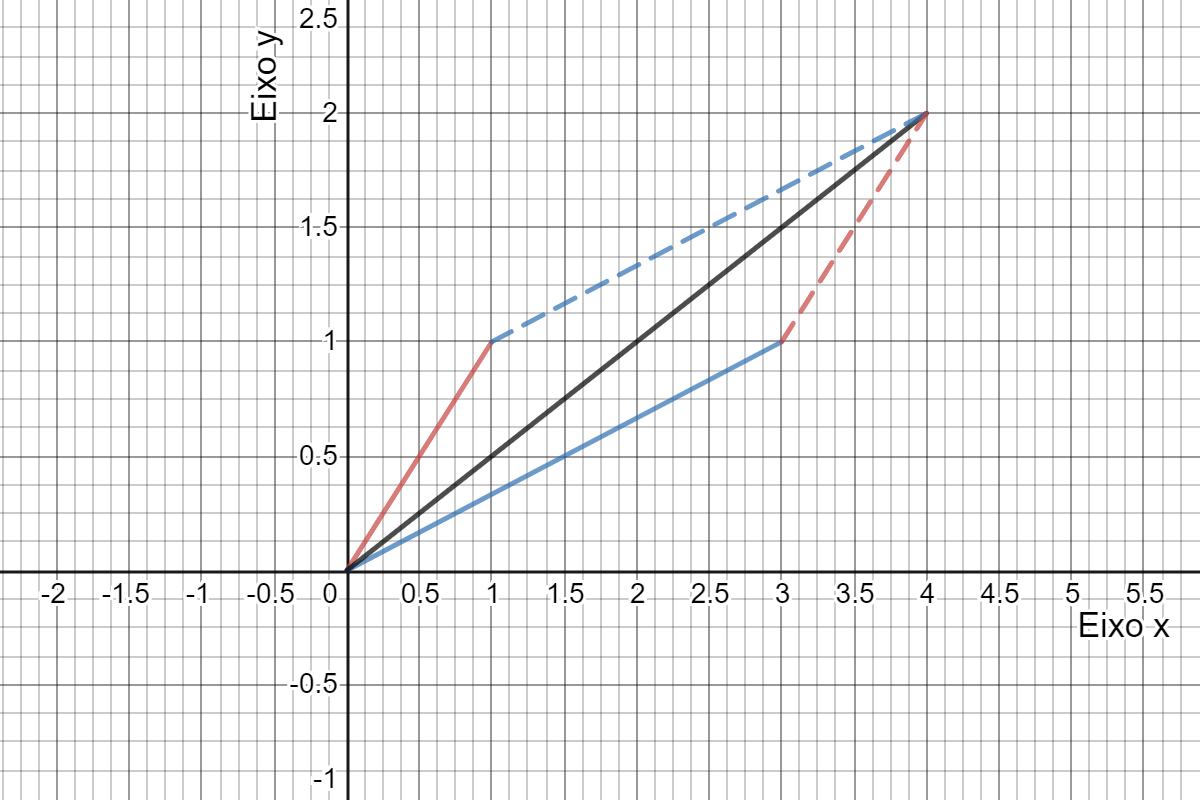
\includegraphics[width=0.6\textwidth]{sum_vectors.png}
    \caption{Representação da soma de vetores usando as flechas e a Regra do Paralelogramo. Em vermelho, é o vetor $\va{a}$, em azul é o vetor $\va{b}$ e, em preto, a soma dos dois vetores $\va{a} + \va{b}$}
    \label{fig:sum_vectors}
\end{figure}

\subsection{Subtração ou Diferença de vetores (-)}

A definição da subtração é bem parecida com a da soma: 
\begin{equation}
    \boxed{\va{a} - \va{b} = (a_1-b_1, a_2-b_2)}
\end{equation}


No nosso caso, seria:

\begin{equation}
    \va{a} - \va{b} = (1-3,1-1) = (-2,0)
\end{equation}

Aqui a ordem da subtração importa, veja a seguir:
\begin{equation}
    \va{b} - \va{a} = (3-1, 1-1) = (2,0)
\end{equation}

Logo, o resultado é outro e o vetor resultante é totalmente diferente. O que diferencia um resultado do outro é qual é o sentido do vetor resultante. Veja as imagens a seguir para ver a diferença.

\begin{figure}[H]
    \centering
    \begin{subfigure}[b]{0.4\textwidth}
         \centering
         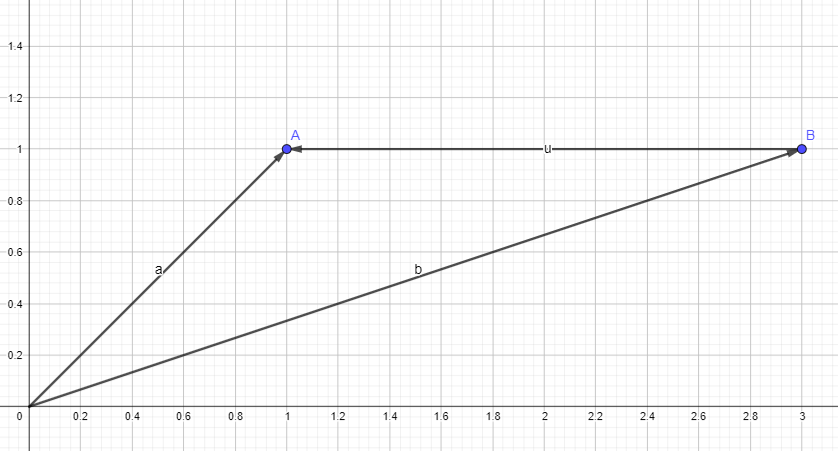
\includegraphics[width=\textwidth]{A-B_vector.png}
         \caption{Demonstração do vetor $\va{a} - \va{b}$ para $\va{a}=(1,1)$ e $\va{b} = (3,1)$. Nesse caso, o vetor resultante é: $\va{u} = \va{a} - \va{b} = (-2,0)$}
         \label{fig:a-b_vec}
     \end{subfigure}
     \hfill
     \begin{subfigure}[b]{0.4\textwidth}
         \centering
         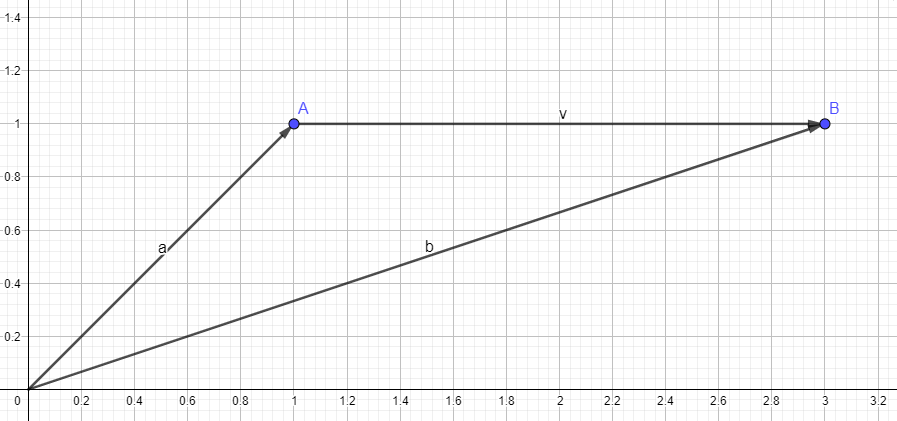
\includegraphics[width=\textwidth]{b-a_vec.png}
         \caption{Demonstração do vetor $\va{b} - \va{a}$ para $\va{a}=(1,1)$ e $\va{b} = (3,1)$. Nesse caso, o vetor resultante é: $\va{v} = \va{b} - \va{a} = (2,0)$}
         \label{fig:b-a_vec}
     \end{subfigure}
    \caption{Demonstração de porque a ordem da subtração muda o sentido do vetor resultante.}
    \label{fig:my_label}
\end{figure}

Aqui nessas figuras está a regra de desenho de vetores para a subtração. \textbf{O vetor resultante começa na ponta do vetor após o sinal de subtração e termina na ponta do vetor antes do sinal!}

\subsection{Comprimento ou Tamanho do vetor ($\norm{\va{a}}$)}

Uma questão interessante sobre o vetor é saber o seu comprimento. Isso nos ajuda a ter uma ideia da intensidade dele. Um exemplo é saber entre 2 carros com velocidades (vetoriais) distintas, qual dele percorre um distância? Para isso, temos uma fórmula para o comprimento de um vetor que é dada por:

\begin{equation}
    \boxed{\norm{\va{a}} = \sqrt{(a_1)^2 + (a_2)^2}}
\end{equation}

\textit{Exemplo:} Dado o vetor $\va{a} = (1,1)$, o tamanho dele é:

\begin{equation}
    \norm{\va{a}} = \sqrt{1^2 + 1^2} = \sqrt{2} 
    \end{equation}
    
\subsection{Multiplicação por escalar}

A última operação que iremos fazer são as multiplicações de um escalar (número) por um vetor. Essa operação é definida da seguinte forma:
\begin{equation}
    \boxed{\alpha \va{a} = \alpha (a_1,a_2) = (\alpha a_1, \alpha a_2)}
\end{equation}
em que $\alpha$ é um número.

\textit{Exemplo:} Dado o vetor $\va{a}=(1,1)$ e $\alpha=-2$, então $\alpha\va{a}$ é:
\begin{equation}
    \alpha\va{a} = (-2)*(1,1) = (-2*1,-2*1) = (-2,-2)
\end{equation}
\end{document}
